\subsection{53 cards}

\renewcommand{\CURPATH}{examples/solitaire/53}

Now take a look on the first part of the loop:

\begin{lstlisting}
.text:0000000100036684 loc_100036684:                          ; CODE XREF: SolitaireGame::InitialDeal(void)+C0↓j
.text:0000000100036684                 mov     eax, 4EC4EC4Fh
.text:0000000100036689                 mul     edi
.text:000000010003668B                 mov     r8d, edx
.text:000000010003668E                 shr     r8d, 4          ; unsigned int
.text:0000000100036692                 mov     eax, r8d
.text:0000000100036695                 imul    eax, 52
.text:0000000100036698                 mov     edx, edi
.text:000000010003669A                 sub     edx, eax        ; unsigned int
.text:000000010003669C                 mov     rcx, [rbx+128h] ; this
.text:00000001000366A3                 call    ?CreateCard@CardTable@@IEAAPEAVCard@@II@Z ; CardTable::CreateCard(uint,uint)
.text:00000001000366A8                 mov     rdx, rax        ; struct Card *
.text:00000001000366AB                 mov     rcx, rbx        ; this
.text:00000001000366AE                 call    ?Push@CardStack@@QEAAXPEAVCard@@@Z ; CardStack::Push(Card *)
.text:00000001000366B3                 inc     edi
.text:00000001000366B5                 cmp     edi, 52
.text:00000001000366B8                 jb      short loc_100036684
\end{lstlisting}

What is with multiplication by 4EC4EC4Fh? Surely, this is division by multiplication.
And what Hex-Rays can say:

\begin{lstlisting}
  v5 = 0;
  do
  {
    v6 = CardTable::CreateCard(v4[37], v5 % 0x34, v5 / 0x34);
    CardStack::Push((CardStack *)v4, v6);
    ++v5;
  }
  while ( v5 < 0x34 );
\end{lstlisting}

Somehow, \verb|CreateCard()| functions takes two arguments: iterator divided by 52 and a remainder of the division operation.
Hard to say, why they did so.
Solitaire can't allow more than 52 cards, so the last argument is senseless, it's always zero.

But when I patch \TT{cmp edi, 52} instruction at 0x1000366B5 to be \TT{cmp edi, 53}, I found that there are now 53 cards.
The last one is \textit{two of clubs}, because it's numbered as 0th card.

During the last iteration, 0x52 is divided by 0x52, remainder is zero, so 0th card is added twice.

What a frustration, there are two \textit{two of clubs}:

\begin{figure}[H]
\centering
\frame{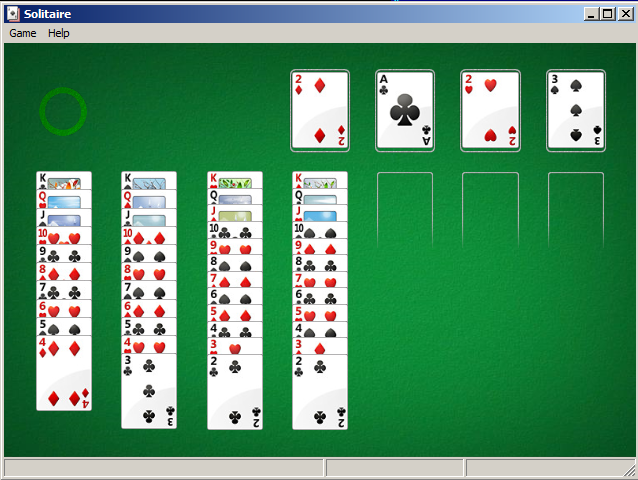
\includegraphics[width=\textwidth]{\CURPATH/1.png}}
\end{figure}

This is patched Windows 7 Solitare:
\href{\RepoURL/examples/solitaire/53/Solitaire53.exe}{Solitaire53}.

